\section{Existing data-intensive computing systems are far from optimal}
\label{sec:benchmarks}

%Published terasort and petasort benchmarks indicate 3-16x longer sort times compared to the optimal performance model.  It includes a results for Grep and TeraSort benchmarks in Figure~\ref{fig:benchmarks1}, results for PetaSort benchmarks in Figure~\ref{fig:benchmarks2}, a more complete listing of the configuration of each system, what our model predicts is the bottleneck resource, and how each system performed as compared to the optimal performance model.

%{
\renewcommand{\baselinestretch}{1.0}
\begin{figure}[t]
\begin{center}

%\resizebox{\columnwidth}{!} {
%   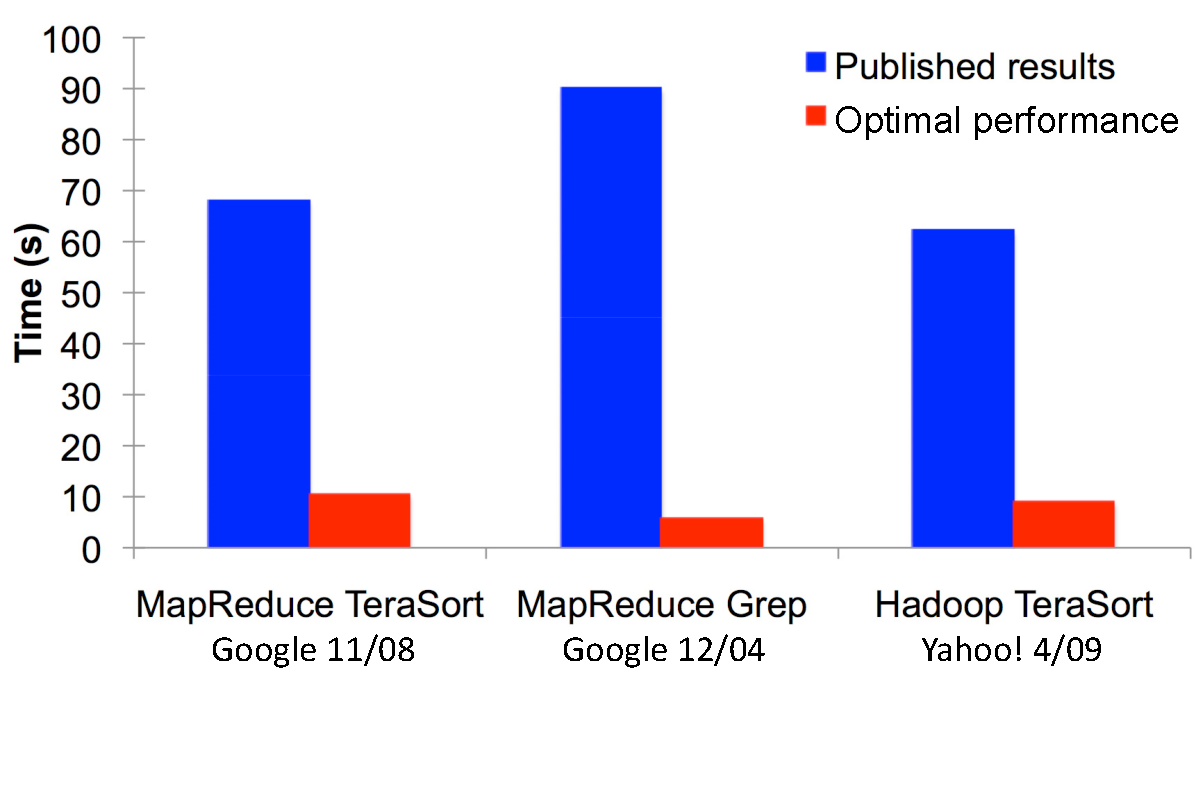
\includegraphics[height=2.5in]{fig_benchmarks1.pdf}
   
\includegraphics[height=2.5in]{pdllogo.eps}
%}

\end{center}
\minicaption{Published benchmarks for Grep and PetaSort}
{
}

\label{fig:benchmarks1}
\end{figure}
}


%
%{
\renewcommand{\baselinestretch}{1.0}
\begin{figure}[t]
\begin{center}

%\resizebox{\columnwidth}{!} {
%   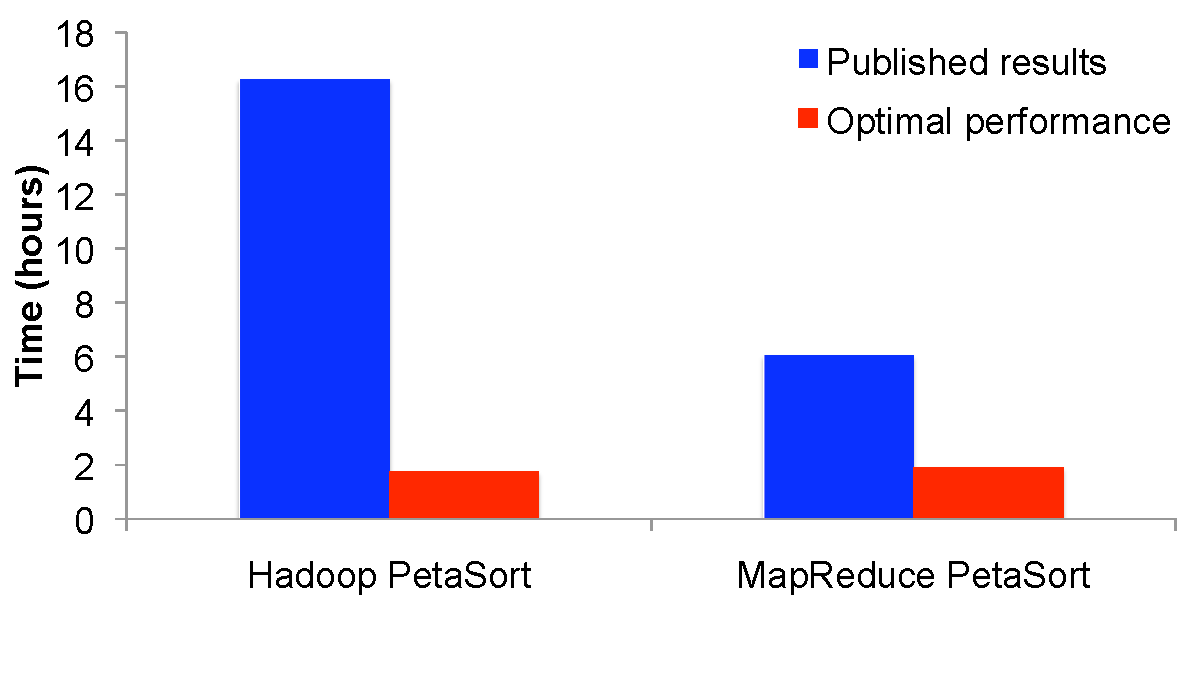
\includegraphics[height=2.5in]{fig_benchmarks2.pdf}
   
\includegraphics[height=2.5in]{pdllogo.eps}
%}

\end{center}
\minicaption{Published benchmarks for TeraSort}
{
}

\label{fig:benchmarks2}
\end{figure}
}




Our model indicates that, though they may scale beautifully, popular
data-intensive computing systems leave a lot to be desired in terms of
efficiency.  Figure~\ref{fig:slowdown} compares optimal times, as
predicted by the model, to reported measurements of a few benchmark
landmarks touted in the literature, presumably on well-tuned instances
of the programming frameworks utilized. These results indicate that
far more machines and disks are often employed than would be needed
if the systems were hardware-efficient.
The remainder of this section describes the systems and benchmarks
represented in Figure~\ref{fig:slowdown}.

%I removed mention of our own experiments on Hadoop for comparison,
%because I think the Hadoop results demonstrate that a lot of
%efficiency is lost at scale, so our 25-node hadoop
%performance isn't a good comparison point for these massive systems

{
\renewcommand{\baselinestretch}{1.0}
\begin{figure}[t]
\begin{center}

   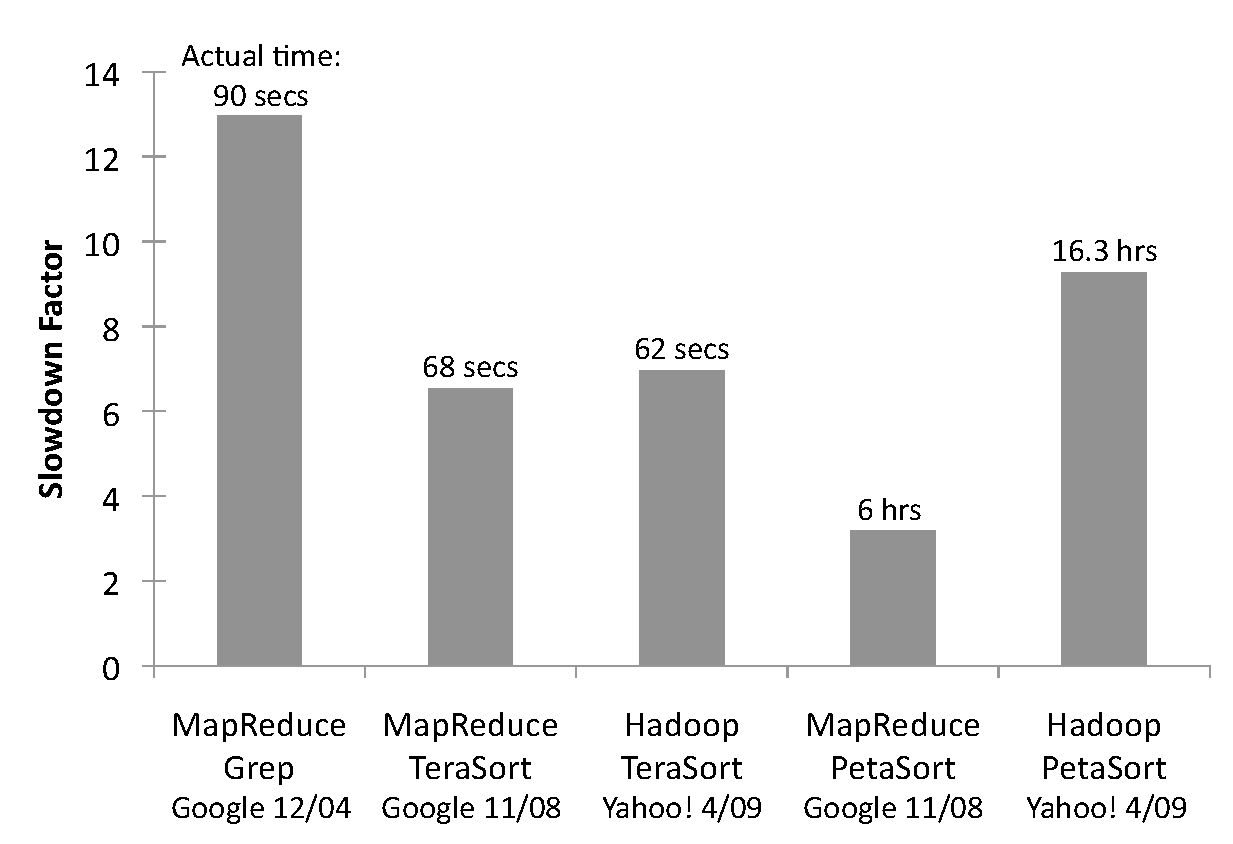
\includegraphics[height=2.5in]{fig_slowdown.eps}

\end{center}
\minicaption{Published benchmarks of popular parallel dataflow
  systems} {Each bar represents the reported throughput relative to
  the ideal throughput indicated by our performance model,
  parameterized according to a cluster's hardware.  }

\label{fig:slowdown}
\end{figure}
}



\minorsection{Hadoop -- TeraSort}
In April 2009,
Hadoop set a new record~\cite{hadoop2009} for sorting 1 TB of data in
the Sort Benchmark \cite{sortbenchmark} format.  The setup had the
following parameters: $i = 1$~TB, $r = 1$,
$n = 1460$, $D = 4$~disks~$\cdot 65$~MB/s/disk $= 260$~MB/s, $N = 110$~MB/s, $d_m = i/n = 685$~MB.
With only 685 MB per node, the data can be sorted by the individual nodes in
memory.
A phase~1 backup write is not needed, given the short runtime.
Equation~\ref{eqn:sortmodel2} gives a best-case runtime of 8.86~seconds.
%A backup write is not beneficial, in this case, so we can apply
%Equation \ref{eqn:sortmodel2} to obtain the optimal execution time:
%\[t_{\textstyle optimal} = \frac{1000000}{1460} \left( \frac{1}{110} + \frac{1}{260}
%\right) = 8.86 \textstyle{ seconds}\]
After fine-tuning the system for this specific
benchmark, Yahoo! achieved
% $t_{\textstyle actual} = 62$
62~seconds---$7\times$ slower.
% than the best-case runtime.
An optimal system using the same hardware would achieve better
throughput with 209 nodes (instead of 1460).

\minorsection{MapReduce -- TeraSort}
In November 2008,
Google reported TeraSort results for 1000 nodes with
12 disks per node~\cite{sorting1pb}. The following parameters were
used: $i = 1$~TB, $r = 1$, $n = 1000$, $D = 12 \cdot 65 = 780$~MB/s,
$N = 110$~MB/s, $d_m = i/n = 1000$~MB.
Equation~\ref{eqn:sortmodel2} gives a best-case runtime of 10.4~seconds.
%As with the Hadoop TeraSort, we can apply
%Equation~\ref{eqn:sortmodel2} to obtain the optimal execution time:
%\[t_{\textstyle optimal} = \frac{1000000}{1000} \left( \frac{1}{110} + \frac{1}{780}
%\right) = 10.37 \textstyle{ seconds}\]
Google achieved
% $t_{\textstyle actual} = 68$
68~seconds---over $6\times$ slower.
% than the best-case runtime.
An optimal system using the same hardware would achieve better
throughput with 153 nodes (instead of 1000).

\minorsection{MapReduce -- PetaSort}
Google's PetaSort experiment~\cite{sorting1pb} is similar to TeraSort,
with three differences:
(1) an external sort is required with a larger
amount of data per node ($d_m = 250$~GB),
(2) output was stored on GFS with three-way replication,
(3) a Phase~1 backup write is justified by the longer runtimes.
In fact, Google ran the experiment multiple times, and at least one disk
failed during each execution.
The setup is described as follows:
$i = 1$~PB, $r = 3$, $n = 4000$, $D = 12 \cdot 65 = 780$~MB/s,
$N = 110$~MB/s, $d_m = i/n = 250$~GB.
The bottom cell of Table~\ref{table:model:replication} gives
a best-case runtime of 6818~seconds.
%Referring to the bottom cell of Table \ref{table:model:replication}:
%\begin{equation}
%t_{\textstyle optimal}
%  = \frac{i}{n} \left( max\left\{\frac{3}{D},
%\frac{1}{N}\right\} + max\left\{\frac{4}{D}, \frac{2}{N}\right\} \right)\\
%%  = \frac{1000000000}{4000} \left( max\left\{\frac{3}{780},
%% \frac{1}{110}\right\} + max\left\{\frac{4}{780}, \frac{2}{110}\right\}
%% \right)\\
%= 6818 \textstyle{ seconds} 
%\end{equation}
Google achieved
% $t_{\textstyle actual} = 21720$
21,720~seconds---approximately $3.2\times$ slower.
% than the best-case runtime.
An optimal system using the same hardware would
achieve better throughput with 1256 nodes (instead of 4000).
Also, according to our model, for the purpose of sort-like
computations, Google's nodes are over-provisioned with disks. In an optimal
system, the network would be the bottleneck even if each node had only 6
disks instead of 12.

%FIXME: Add reasons for google over-provisioning?

\minorsection{Hadoop -- PetaSort}
Yahoo!'s PetaSort experiment~\cite{hadoop2009} is similar to Google's,
with one
difference: The output was stored on HDFS with two-way replication.
The setup is described as follows: $i = 1$~PB, $r = 2$, $n = 3658$, $D = 4 \cdot 65 = 260$~MB/s,
$N = 110$~MB/s, $d_m = i/n = 273$~GB.
The bottom cell of Table~\ref{table:model:replication} gives
a best-case runtime of 6308~seconds.
%\begin{equation}
%t_{\textstyle optimal} = \frac{i}{n} \left( max\left\{\frac{3}{D}, \frac{1}{N}\right\} + max\left\{\frac{3}{D}, \frac{1}{N}\right\} \right)\\
%%  = \frac{1000000000}{3658} \left( max\left\{\frac{3}{260}, \frac{1}{110}\right\} + max\left\{\frac{3}{260}, \frac{1}{110}\right\} \right)\\
%  = 6308.6 \textstyle{ seconds}
%\end{equation}
Yahoo! achieved
% $t_{\textstyle actual} = 58500$
58,500~seconds---about $9.3\times$
slower.
% than the best-case runtime.
An optimal system using the same hardware would achieve better
throughput with 400 nodes (instead of 3658).

\minorsection{MapReduce -- Grep}
The original MapReduce paper \cite{mapreduce} described a distributed grep
computation that was executed on MapReduce. The setup is described
as follows: $i = 1$~TB, $n = 1800$, $D = 2 \cdot 40 = 80$~MB/s,
$N = 110$~MB/s, $d_m = 9.2$~MB, $e_M = 9.2/1000000 \approx 0$, $e_R = 1$.
The paper does not specify the throughput of the disks, so we used 40 MB/s,
conservatively estimated based on disks of the timeframe (2004).
Equation \ref{eqn:grepmodel} gives a best-case runtime of 6.94~seconds.
%these parameters is:
%\[t_{\textstyle optimal} = \frac{i}{n D} = 5.56 \textstyle{ seconds}\]
Google achieved
% $t_{\textstyle actual} = 150$
150~seconds including startup overhead,
or 90~seconds without that overhead---still about $13\times$ slower.
% than the best-case runtime.
An optimal system using the same hardware would achieve better
throughput with 139 nodes (instead of 1800).
The 60-second startup time experienced by MapReduce on a
cluster of 1800 nodes would also have been much shorter on a
cluster of 139 nodes.


%\minorsection{MapReduce -- OLD HADOOP?}
%Elie had noted "older Hadoop TeraSort~\cite{hadoop2008}"... what do we
%know about it?

%\minorsection{MapReduce -- our Hadoop?}
%This may be going in the other section, but here's a placeholder just
%in case.

%ekrevat: moved sources of inefficiency into the discussion section
